% Section content template for individual Educative lessons
% This file contains the actual content for a specific section
% Generated from Educative API section content

% Section: Activity Diagram for the Elevator System
% Section ID: 6452401311842304
% Section Slug: activity-diagram-for-the-elevator-system
% Generated: 2025-12-11T14:08:46.082036

An activity diagram is a great way to visualize the flow of messages from one activity to another in the system. There can be different activity diagrams that we can create for our elevator system. In this lesson, we will create activity diagrams for the following two activities:

\begin{itemize}
\item
\protect\phantomsection\label{pH8RKZFsThP7y8zfrPo0C}
The passenger arrives at the desired floor.
\item
\protect\phantomsection\label{r56wM3OHLjthWutL3O5CJ}
\textbf{Activity challenge:} The passenger calls for the elevator.
\end{itemize}

\subsection{The passenger arrives at the desired floor}\label{OTOyJ6rT_pOQBegLwU4as}
\\
The following are the states and actions that will be involved in this activity diagram.

\subsubsection{States}\label{0mbDpwXhm2w4q8AoSWY_O}
\\
\textbf{Initial state:} The passenger enters the elevator car.
\\
\textbf{Final state:} There are two final states present in this activity diagram. These are shown below:

\begin{itemize}
\item
\protect\phantomsection\label{HPMCYACBp6ZvNgpUg5GG9}
The passenger arrives at the destination floor.
\item
\protect\phantomsection\label{-VZrMMApRwtaJ54YG-Cuq}
The passenger is not allowed due to max load/capacity issues.
\end{itemize}

\subsubsection{Actions}\label{Dy9Fn49wIazUsHmstoTza}
\\
The passenger enters the elevator car, checks to see if the safety limits are met, stops at other passengers' floors, and finally reaches the desired floor.
\\
Based on the order above, the activity diagram of a passenger arriving at their desired floor is given below.
\begin{quote}
\textbf{Note:} The passenger is just entering the elevator, so either the up or the down button can be pressed.
\end{quote}

\begin{figure}[htbp]
 \centering
 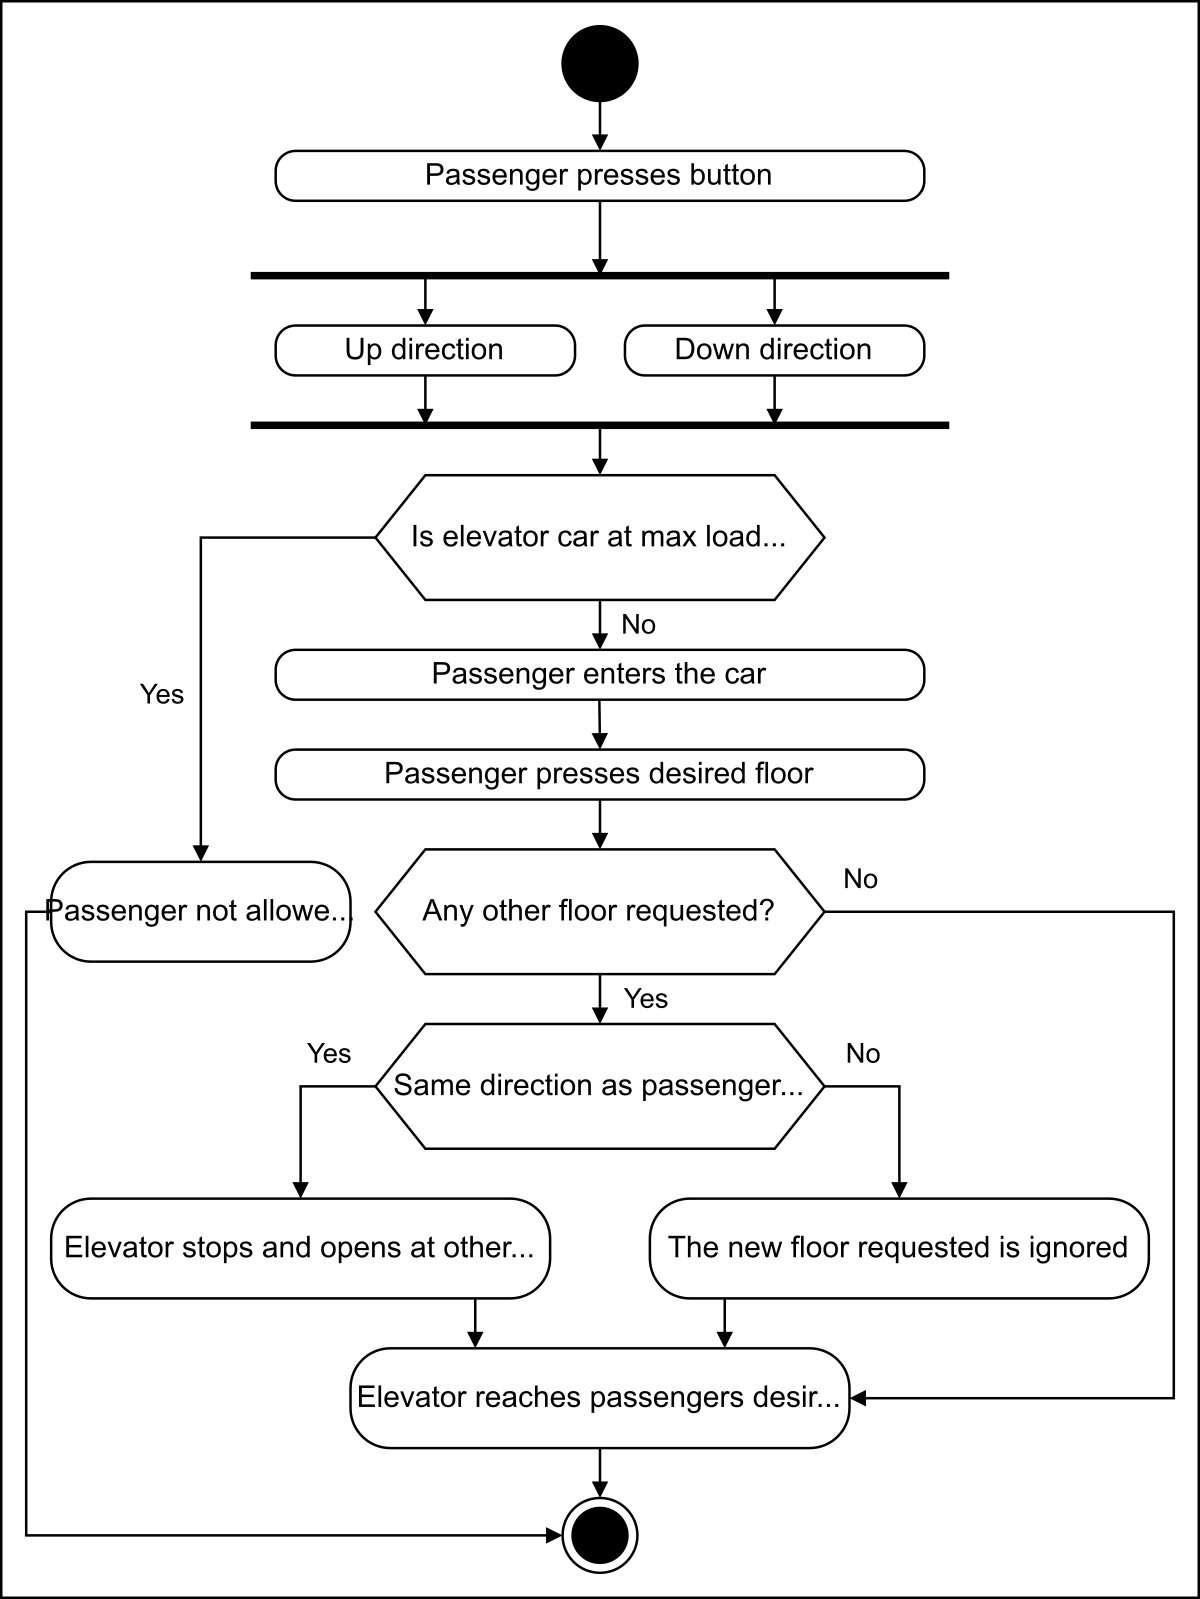
\includegraphics[width=0.5\textwidth]{Images/chapter_8/section_6452401311842304/5560011004837888.png}
 \caption{The activity diagram for a passenger arriving at their desired floor}
\end{figure}

\subsection{Activity challenge: The passenger calls for the elevator}\label{g4wltaawkZ9h9xG7OHqGv}
\\
You will create an activity diagram of a passenger calling for the elevator.
\\
A skeleton of the activity diagram is given below.

\begin{figure}[htbp]
 \centering
 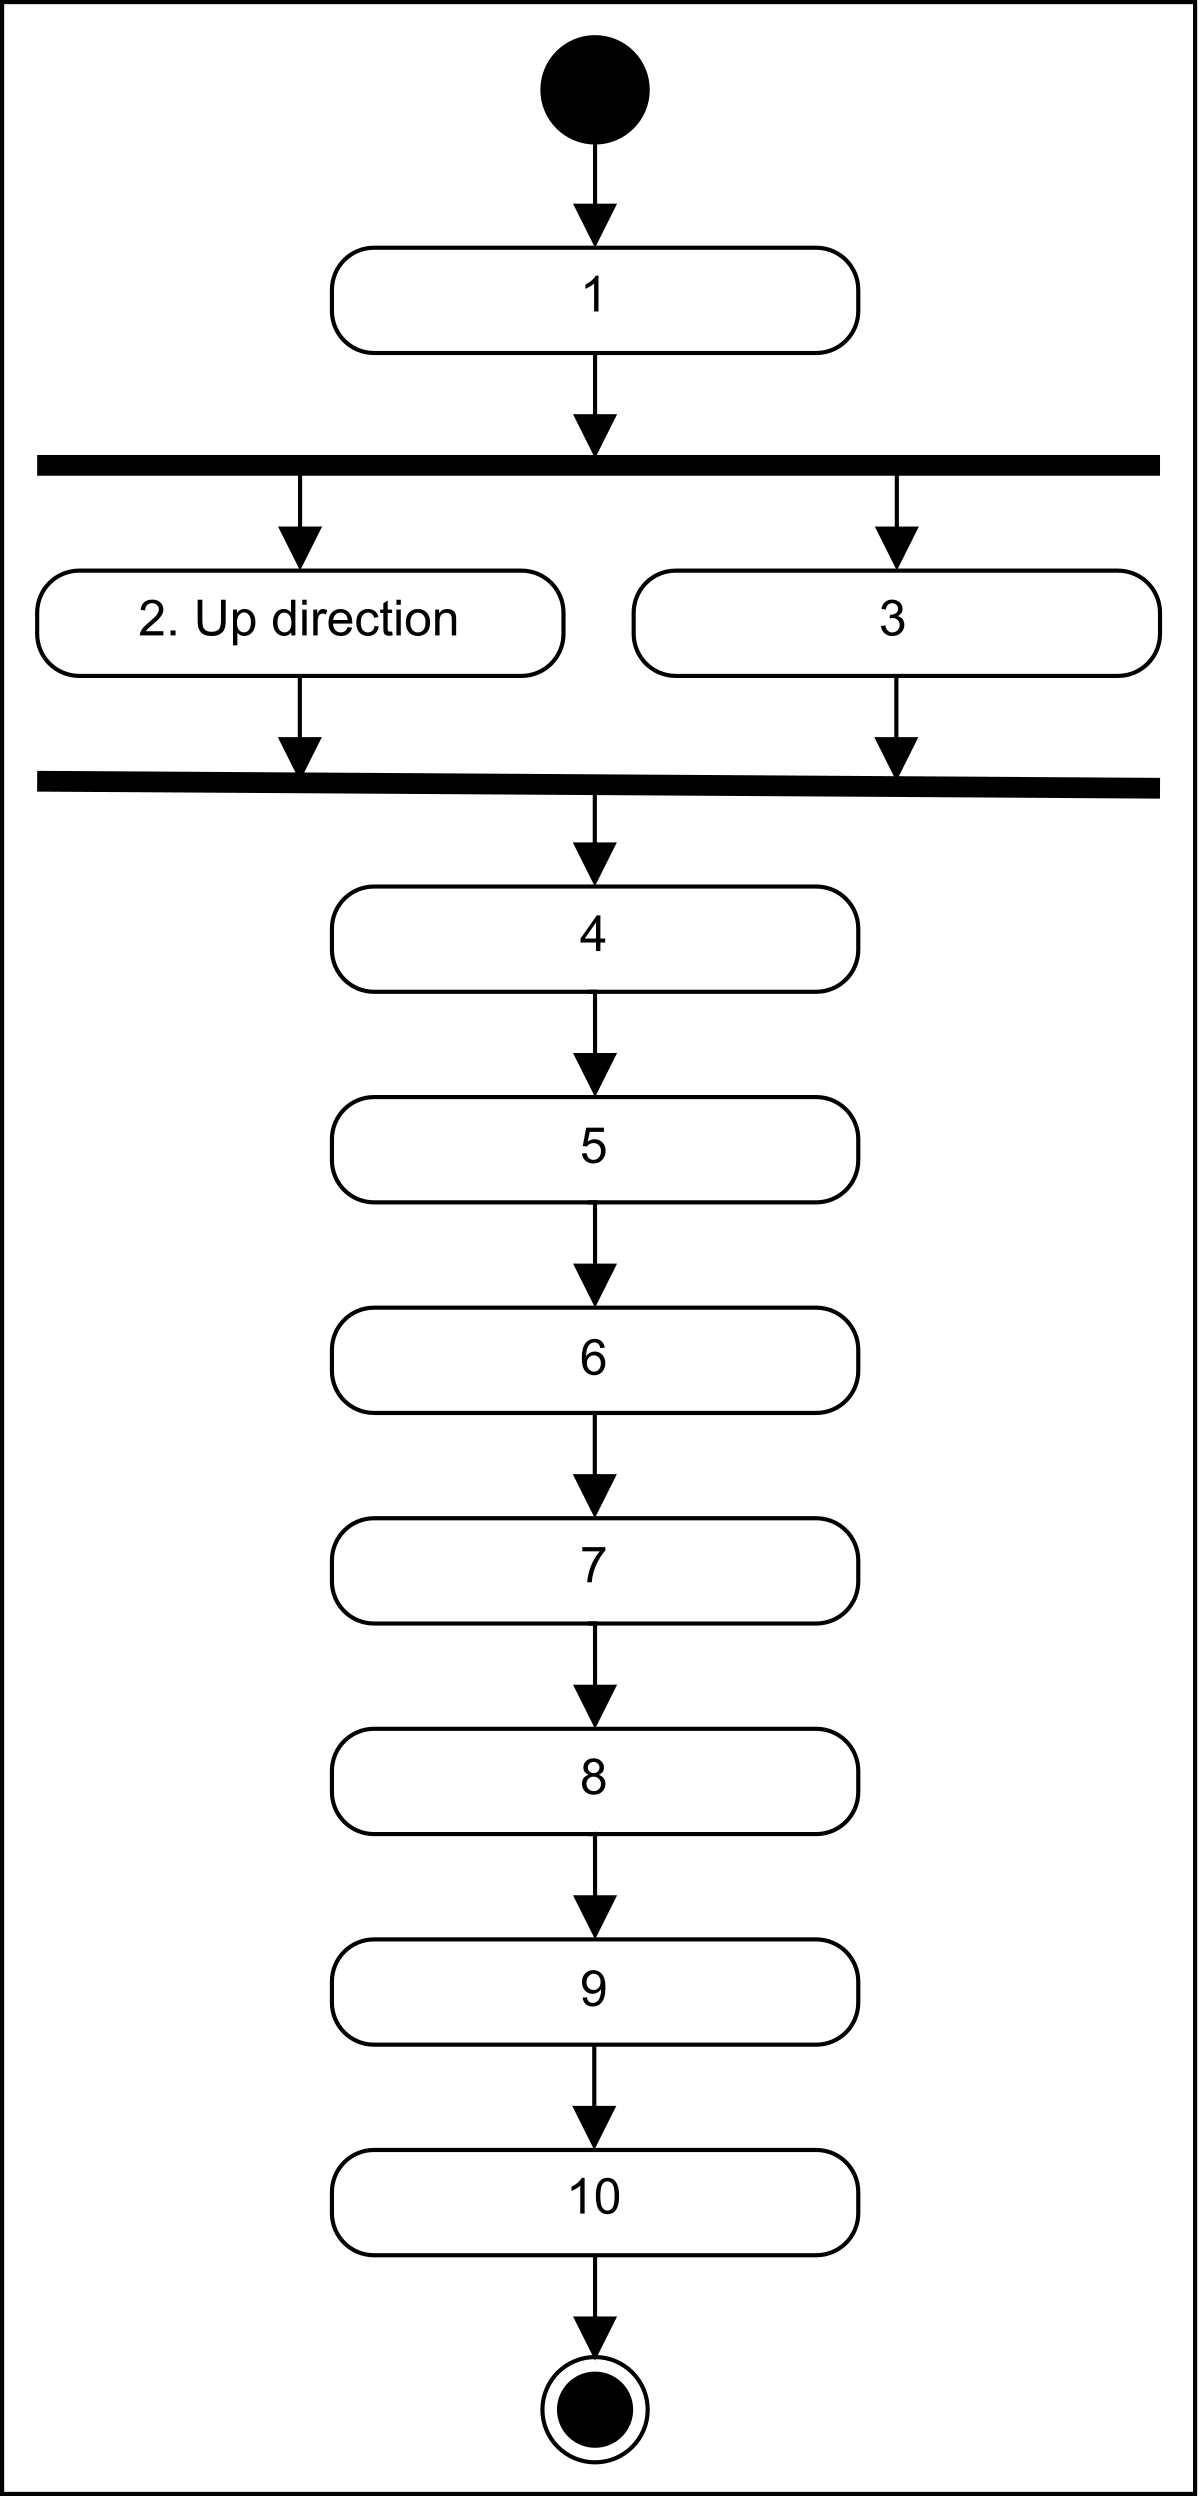
\includegraphics[width=0.25\textwidth]{Images/chapter_8/section_6452401311842304/4957111144677376.png}
 \caption{The activity diagram for a passenger calling for the elevator}
\end{figure}

Notice that the actions in the diagram above are numbered from 1 to 10. The slots below represent the activities, and the arrows represent the flow from one activity to another.
\\
Can you rearrange the slots below in the correct order they should appear in the activity diagram above?
\begin{quote}
\textbf{Note:}~If you're stuck, click the ``Show Solution'' button.
\end{quote}

Alternatively, you can also click the ``Show complete diagram'' button below to see the complete sequence diagram.

We've looked at some of the activity diagrams of our elevator system. In the next lesson, we will present the code for our designed classes in some of the most popular languages.

% End of section content